\chapter{TINJAUAN PUSTAKA}
\vspace{1ex}

\section*{}
Demi mendukung penelitian ini, dibutuhkan beberapa teori penunjang sebagai bahan acuan dan referensi. Dengan demikian penelitian ini menjadi lebih terarah. 
\vspace{1ex}

\section{3D Convolutional Neural Network (3D-CNN)}
\vspace{1ex}

\begin{figure} [!htb]
	\captionsetup{justification=centering}
	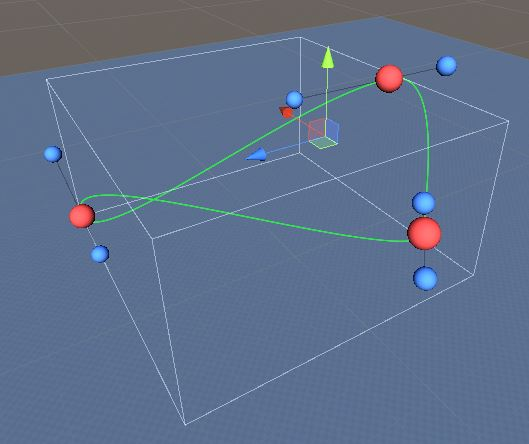
\includegraphics[scale=0.4]{img/contoh-kurva-bezier.JPG}
	\caption{Contoh kurva bezier pada bidang 3 dimensi}
	\label{fig:2.1}
\end{figure}

\textit{3D Convolutional Neural Network} adalah suatu arsitektur neural network dimana mengekstrak fitur dari dimensi spasial dan temporal dengan melakukan konvolusi 3D, sehingga menangkap informasi gerakan yang dikodekan dalam beberapa bingkai yang berdekatan. Arsitektur yang digunakan menghasilkan banyak saluran informasi dari bingkai masukan, dan representasi fitur akhir menggabungkan informasi dari semua saluran.
\vspace{1ex}

\section{\textit{Embedded System} atau Sistem Tertanam}
\vspace{1ex}

\begin{figure} [!htb]
	\captionsetup{justification=centering}
	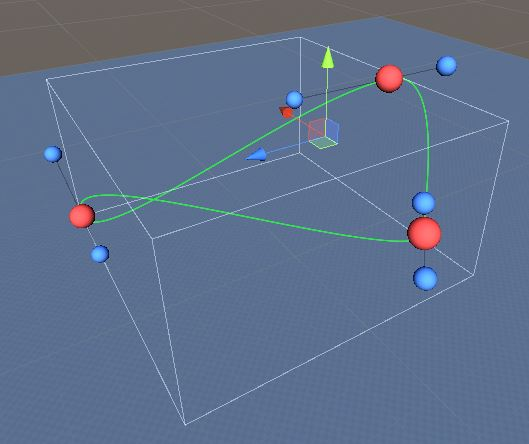
\includegraphics[scale=0.4]{img/contoh-kurva-bezier.JPG}
	\caption{Contoh kurva bezier pada bidang 3 dimensi}
	\label{fig:2.1}
\end{figure}

\textit{Embedded System} adalah suatu system pengolah informasi yang digabungkan atau ditanamkan ke suatu produk atau benda lain. Sistem pengolah informasi di sini tidak harus berupa komputer atau mikroprosesor. Tertanam atau menyatu di sini berarti bagi orang yang melihat produk hanya melihat produk saja, tidak lagi melihat prosesor di dalamnya sebagai suatu benda yang terpisah.
\vspace{1ex}
